% Machine translated from the Danish original, ../danish/ad-problems-2023-april.tex
% From the front page: CLRS refers to the course textbook, Introduction to Algorithms, 3rd edition.
\noindent\emph{This problem set has been machine translated from the Danish original.}
\medskip

\section*{Multiple-choice}\label{sec:mc}

\placeholder{Where to enter the multiple-choice answers, e.g.\ the multiple-choice module of the exam system.}

\multiplechoicestart

\question{MergeSort and recursion}
If {\sc MergeSort}$(A,p,r)$, implemented as in CLRS Section 2.3,
is called on 4 elements (i.e., $r-p+1 = 4$), the first recursive call is made on a list of 2 elements, from which the first recursive call is made on a list with 1 element. So at the time we reach the bottom of the recursion there are 3 calls of {\sc MergeSort} on the recursion stack at the same time.
If {\sc MergeSort}$(A,p,r)$ is called on 5 elements, there are up to 4 simultaneous calls on the recursion stack.

\medskip

Now suppose that {\sc MergeSort}$(A,p,r)$ is called on 42 elements (i.e., $r-p+1 = 42$).
What is the largest number of simultaneous calls to {\sc Merge-Sort}, i.e., the number of calls on the recursion stack?
\oneanswer
\optionsstart
\answer 3 simultaneous calls.
\answer 4 simultaneous calls.
\answer 5 simultaneous calls.
\answer 6 simultaneous calls.
\answer 7 simultaneous calls. \correct
\optionsend
\explanation{The largest number of elements in a call at recursion depth 1,2,3,\dots\ is 42, 21, 11, 6, 3, 2 and 1, respectively. So there are up to 7 simultaneous calls.}


\question{Shortest-paths tree}
Consider a single-source shortest-paths problem on a directed graph $G=(V,E)$ with weight function $w: E\rightarrow \mathbb{R}$ and source vertex $s$.
Which of the following properties does a shortest-paths tree $G'=(V',E')$ always have?
\multipleanswers
\optionsstart
\answer Every path in $G'$ is a shortest path in $G$. \correct
\answer Every shortest path in $G$ corresponds to a path in $G'$.
\answer $G'$ is a binary tree with $s$ as its root.
\answer $G'$ is a minimum spanning tree.
\answer It can be computed with Dijkstra's algorithm.
\optionsend
\explanation{There may be several shortest paths between $s$ and a vertex $v$ (with the same weight), and the shortest-paths tree contains exactly one of them.
The shortest-paths tree is not necessarily binary; for example, we can have a graph where every shortest path from $s$ consists of a single edge, i.e., $s$ has edges to $|V'|-1$ vertices.
A minimum spanning tree (MST) minimizes the sum of edge weights and does not necessarily contain the shortest paths from a particular vertex $s$; consider, e.g., an undirected graph with three vertices and edges of weight 2, 2 and 3, where an MST contains the two edges of weight 2, but where the edge of length 3 is the shortest path between two of the vertices.
Dijkstra's algorithm is only guaranteed to be correct when there are no negative weights, so if this is not the case the output may be wrong. (Instead one can use another algorithm, e.g., Bellman-Ford.)
}


\question{Shortest paths}
Consider the single-source shortest-paths problem with source vertex {\bf a} on the following graph:\newline
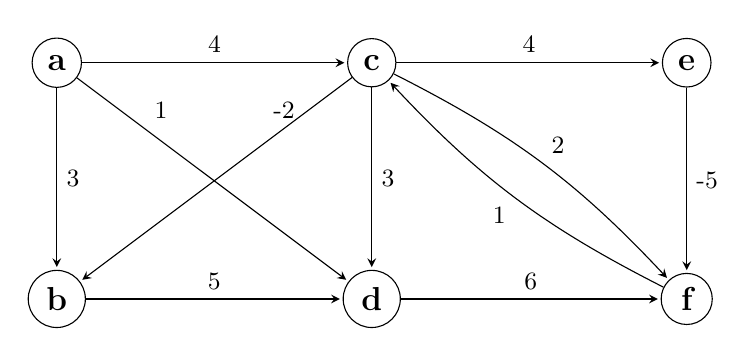
\begin{tikzpicture}[->,>=stealth,shorten >=1pt,auto,
    main node/.style={circle,draw,font=\large\bfseries}]
\node[main node] (a) at (2,1.5) {a};
\node[main node] (b) at (2,-1.5) {b};
\node[main node] (c) at (6,1.5) {c};
\node[main node] (d) at (6,-1.5) {d};
\node[main node] (e) at (10,1.5) {e};
\node[main node] (f) at (10,-1.5) {f};

\path[every node/.style={font=\small}]
(a) edge node {3} (b)
edge node {4} (c)
edge node[pos=0.25] {1} (d)
(b) edge node {5} (d)
(c) edge node {3} (d)
edge [bend left=10] node {2} (f)
edge node {4} (e)
edge node[pos=0.25, above] {-2} (b)
(d) edge node {6} (f)
(e) edge node {-5} (f)
(f) edge [bend left=10] node {1} (c);
\end{tikzpicture}\\
Which edges are in the shortest-paths tree?
\multipleanswers
\optionsstart
\answer (a,b)
\answer (a,c) \correct
\answer (a,d) \correct
\answer (b,d)
\answer (c,b) \correct
\answer (c,d)
\answer (c,e) \correct
\answer (c,f)
\answer (d,f)
\answer (e,f) \correct
\answer (f,c)
\optionsend
\explanation{Since there are negative weights, the edges of the tree can be found by running the Bellman-Ford algorithm, which gives the output indicated (which is unique in this case).}



\question{Prim's algorithm}
Consider the following weighted, undirected graph:
\begin{center}
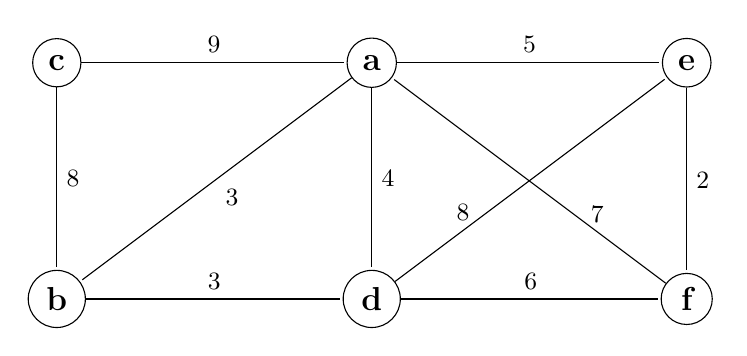
\begin{tikzpicture}[-,>=stealth,shorten >=1pt,auto,
    main node/.style={circle,draw,font=\large\bfseries}]
\node[main node] (a) at (6,1.5) {a};
\node[main node] (b) at (2,-1.5) {b};
\node[main node] (c) at (2,1.5) {c};
\node[main node] (d) at (6,-1.5) {d};
\node[main node] (e) at (10,1.5) {e};
\node[main node] (f) at (10,-1.5) {f};

\path[every node/.style={font=\small}]
(a) edge node {3} (b)
edge node {5} (e)
edge node {4} (d)
(b) edge node {3} (d)
(c) edge node {9} (a)
edge node {8} (b)
(d) edge node {6} (f)
edge node [pos=0.25, above]{8} (e)
(e) edge node {2} (f)
(f) edge node [pos=0.25, above]{7} (a) ;
\end{tikzpicture}
\end{center}
If Prim's algorithm is run on this graph starting at vertex {\bf a}, in which order are the vertices included in the minimum spanning tree? (In other words, in which order are they extracted from the priority queue?)
\oneanswer
\optionsstart
\answer a, b, d, e, f, c \correct
\answer a, b, e, d, f, c % Dijkstra
\answer a, b, d, c, f, e % Sorted by weight
\answer a, b, e, f, d, c % Greedy
\optionsend
\explanation{Running Prim's algorithm by hand gives the order indicated. Note that the order is \emph{not} the same as for Dijkstra's shortest-paths algorithm.}



\question{Minimum spanning tree}
Consider the minimum spanning tree problem on the following weighted, undirected graph:\newline
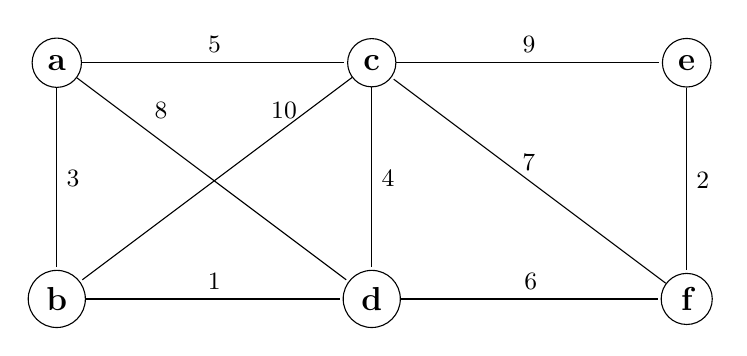
\begin{tikzpicture}[-,>=stealth,shorten >=1pt,auto,
    main node/.style={circle,draw,font=\large\bfseries}]
\node[main node] (a) at (2,1.5) {a};
\node[main node] (b) at (2,-1.5) {b};
\node[main node] (c) at (6,1.5) {c};
\node[main node] (d) at (6,-1.5) {d};
\node[main node] (e) at (10,1.5) {e};
\node[main node] (f) at (10,-1.5) {f};

\path[every node/.style={font=\small}]
(a) edge node {3} (b)
edge node {5} (c)
edge node[pos=0.25] {8} (d)
(b) edge node {1} (d)
(c) edge node {4} (d)
edge node {9} (e)
edge node[pos=0.25, above] {10} (b)
(d) edge node {6} (f)
(e) edge node {2} (f)
(f) edge node[above] {7} (c);
\end{tikzpicture}\\
Which edges are in a minimum spanning tree?
\multipleanswers
\optionsstart
\answer \{a,b\} \correct
\answer \{a,c\}
\answer \{a,d\}
\answer \{b,d\} \correct
\answer \{c,b\}
\answer \{c,d\} \correct
\answer \{c,e\}
\answer \{c,f\}
\answer \{d,f\} \correct
\answer \{e,f\} \correct
\optionsend
\explanation{A minimum spanning tree can be found by running, e.g., Kruskal's or Prim's algorithm, which gives the output indicated (which is unique in this case).}


\question{Cuts and safe edges}
Consider the following undirected, weighted graph with vertex set $V=\{a,b,c,d,e,f\}$:\\
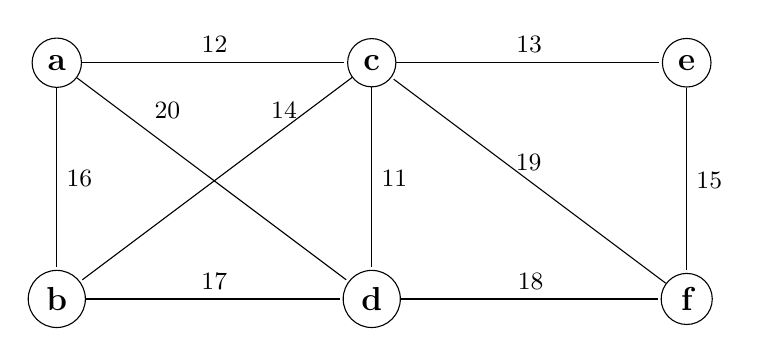
\begin{tikzpicture}[-,>=stealth,shorten >=1pt,auto,
    main node/.style={circle,draw,font=\large\bfseries}]
\node[main node] (a) at (2,1.5) {a};
\node[main node] (b) at (2,-1.5) {b};
\node[main node] (c) at (6,1.5) {c};
\node[main node] (d) at (6,-1.5) {d};
\node[main node] (e) at (10,1.5) {e};
\node[main node] (f) at (10,-1.5) {f};

\path[every node/.style={font=\small}]
(a) edge node {16} (b)
edge node {12} (c)
edge node[pos=0.25] {20} (d)
(b) edge node {17} (d)
(c) edge node {11} (d)
edge node {13} (e)
edge node[pos=0.25, above] {14} (b)
(d) edge node {18} (f)
(e) edge node {15} (f)
(f) edge node[above] {19} (c);
\end{tikzpicture}\\
Consider the edge set $A= \{\{a,c\},\{c,d\}\}$, which is a subset of a minimum spanning tree.
We are interested in cuts, safe edges for $A$, and cuts that respect an edge set $A$. Which of the following statements are true?
\multipleanswers
\optionsstart
\answer Let $S_1=\{a,b,c,d\}$. The cut $(S_1,V - S_1)$ respects the edge set $A$. \correct
\answer Let $S_2=\{a,c,e\}$. The cut $(S_2,V - S_2)$ respects the edge set $A$.
\answer Let $S_3=\{b,e,f\}$. The cut $(S_3,V - S_3)$ respects the edge set $A$. \correct
\answer $\{d,f\}$ is a safe edge for $A$.
\answer $\{c,e\}$ is a safe edge for $A$. \correct
\answer $\{a,d\}$ is a safe edge for $A$.
\optionsend
\explanation{ The edge $\{c,d\}$ crosses the cut $(S_2,V - S_2)$, so it does not respect $A$.
The cuts with $S_1$ and $S_3$ have no edge of $A$ crossing them, so they respect $A$.
The edge $\{d,f\}$ does not have minimum weight in the cut $(\{a,c,d\},\{b,e,f\})$, so it is not safe.
The edge $\{c,e\}$ has minimum weight in the cut $(\{a,c,d\},\{b,e,f\})$, so it is safe.
The edge $\{a,d\}$ does not cross the cut $(\{a,c,d\},\{b,e,f\})$, so it is not safe.
}


\question{Amortized analysis}
In this problem we consider the potential function used to analyze a binary counter in CLRS Section 17.3.
Let $\Phi(D_i)$ denote the value of the potential function after $i$ {\sc Increment} operations.
Which properties does $\Phi(D_i)$ have?
(Note that the statements are not independent --- if $f(i) = \Omega(i)$ holds, then $f(i) = \Omega(\lg i)$ also holds, etc.)
\multipleanswers
\optionsstart
%\answer $\Phi(D_i) = \Omega(1)$. \correct Omitted since the potential becomes 0 when i=2^k
\answer $\Phi(D_i) = \Omega(\lg i)$.
\answer $\Phi(D_i) = \Omega(i)$.
\answer $\Phi(D_i) = O(1)$.
\answer $\Phi(D_i) = O(\lg i)$. \correct
\answer $\Phi(D_i) = O(i)$. \correct
\optionsend
\explanation{ $\Phi(D_i)$ equals the number of 1s in the binary representation of the number $i$ (which is at least 1 for $i>0$). If $i$ is a power of 2, then $\Phi(D_i) = 1$, so we cannot bound the function from below by an increasing function of $i$. If $i+1$ is a power of 2, then $\Phi(D_i) = \lg(i+1)$, so both $O(\lg i)$ and $O(i)$ are valid upper bounds.
}



\question{Running time}
Consider the following code in the pseudocode notation of CLRS:
\begin{codebox}
 \Procname{$\proc{Loops}(n)$}
 \li $r = 0$
 \li \For $i = 1$ \To $n/2$
 \li \Do \For $j = n/2-i$ \To $n$
 \li \Do $r = r + j$ \End \End \End
 \li \Return r
\end{codebox}
We assume that $n/2$ is an integer, so that the outer {\bf for} loop has $n/2$ iterations.
Which of the following are valid statements about the running time $T(n)$ of {\sc Loops}$(n)$?
(Note that the statements are not independent --- if $f(n) = O(n)$ holds, then $f(n) = O(n \lg n)$ also holds, etc.)
\multipleanswers
\optionsstart
\answer $T(n) = O(n)$.
\answer $T(n) = O(n \lg n)$.
\answer $T(n) = O(n^2)$. \correct
\answer $T(n) = \Omega(n)$. \correct
\answer $T(n) = \Omega(n \lg n)$. \correct
\answer $T(n) = \Omega(n^2)$. \correct
\optionsend

\explanation{ There are $n/2$ iterations of the outer loop, each taking $O(n)$ time because the inner loop makes between $n/2$ and $n$ iterations. So the running time is $\Theta(n^2)$. Hence the first two big-O bounds are too low, while the remaining bounds hold.}



\question{Recurrences}
Which of these recurrences have the solution
$T(n) = \Theta(n \lg n)$? Assume that $T(n)=1$ for $n\leq 1$.
\multipleanswers
\optionsstart
\answer $T(n) = 2 T(\lfloor n/2\rfloor ) + n^2$.
\answer $T(n) = 2 T(\lfloor n/2\rfloor ) + 3n$. \correct
\answer $T(n) = 2 T(\lfloor n/3\rfloor ) + 2n$.
\answer $T(n) = 3 T(\lfloor n/2\rfloor ) + n \lg n$.
\answer $T(n) = 3 T(\lfloor n/3\rfloor ) + n$. \correct
\answer $T(n) = T(n-1) + \lg n$. \correct % Cannot be solved with the master theorem in CLRS
\optionsend
\explanation{ The first five recurrences can be solved using the master theorem, where numbers 2 and 5 fall in case 2 and give $T(n) = \Theta(n \lg n)$.
The last recurrence can be solved with the substitution method, where there are $n$ terms of size at most $\lg n$, and where half of them have size at least $\lg(n/2) = \lg(n) - 1$.
}



\question{Divide and conquer}
Suppose you have a recursive algorithm $A$, and let $n$ denote the size of the algorithm's input~$X$.
If $n=1$, the result $A(X)$ is computed in constant time.
For $n>1$ the algorithm first spends $O(n \lg n)$ time computing four inputs $X_1, X_2, X_3, X_4$, each of size $\lfloor n/2\rfloor$, and $A(X_1), A(X_2), A(X_3), A(X_4)$ are computed recursively.
Finally, the recursive answers are combined into an output $A(X)$ in time $O(n^2)$.

\medskip

Which of these recurrences describes the running time $T(n)$ of $A$ on input $X$?
\oneanswer
\optionsstart
\answer $T(n) = 4 T(\lfloor n/2\rfloor ) + O(n \lg n)$.
\answer $T(n) = 2 T(\lfloor n/4\rfloor ) + O(n \lg n)$.
\answer $T(n) = 4 T(\lfloor n/2\rfloor ) + O(n^2)$. \correct
\answer $T(n) = 2 T(\lfloor n/4\rfloor ) + O(n^2)$.
\optionsend
\explanation{ The four recursive subproblems of size $\lfloor n/2\rfloor$ take total time $4 T(\lfloor n/2\rfloor )$. In addition, a total of $O(n^2)$ time is spent computing $A(X)$.
}



\question{Fibonacci heaps}
Consider a Fibonacci heap $H$, as described in CLRS Chapter 19, on which $n_1$ {\sc Insert} operations, $n_2$ {\sc Extract-Min} operations, and $n_3$ {\sc Decrease-Key} operations are performed.
The total number of operations is $n=n_1+n_2+n_3$.
Which of the following statements are always true?
\multipleanswers
\optionsstart
\answer The total worst-case time for the operations is $\Omega(n \lg n)$.
\answer The total worst-case time for the operations is $O(n \lg n)$. \correct
\answer The total worst-case time for the operations is $O(n_1 + n_3 + n_2 \lg n)$. \correct
\answer $H$ has $n_1 - n_2 - n_3$ nodes.
\answer $H$ has $m(H) = n_1 - n_2$ marked nodes.
\optionsend
\explanation{ The amortized analysis gives an upper bound of $O(n_1 + n_3 + n_2 \lg n)$ for the operations. Since $n=n_1+n_2+n_3$, this is in particular $O(n \lg n)$. If $n_1 + n_3 > n_2\lg n$, the time becomes $O(n)$, so the time is not necessarily $\Omega(n \lg n)$. The number of nodes in $H$ is the number of insertions minus the number of deletions, i.e., $n_1 - n_2$, which differs from $n_1 - n_2 - n_3$ if $n_3 >0$.
The number of marked nodes cannot be expressed in terms of $n_1$ and $n_2$ --- for example, {\sc Insert} does not change the number of marked nodes.
}



\question{Binary search trees}\label{q:red-black}
Consider a red-black binary search tree $T$, as described in CLRS Chapter 13.
Consider the tree below, where all leaves are omitted (as in CLRS Figure 13.1(c)) and two internal nodes are unspecified:

\begin{center}
\begin{tikzpicture}[-,>=stealth,level/.style={sibling distance = 5cm/#1,
    level distance = 1cm}]
  \node [black] {42}
      child{ node [red] {24}
              child{ node [black] {19}
                  child{ node [red] {14} }
                  child{ node [white] {}}
              }
              child{ node [gray] {?}
                              child{ node [red] {27}}
                              child{ node [red] {31}}
              }
      }
      child{ node [black] {56}
              child{ node [red] {47}
              }
              child{ node [white] {?}
              }
          }
  ;
  \end{tikzpicture}
\end{center}

\medskip

Which nodes are possible in at least one of the positions marked with ?, if the tree must satisfy the invariants of a red-black binary search tree?
\multipleanswers
\optionsstart
\answer A red node with key 28.
\answer A red node with key 44.
\answer A red node with key 58. \correct
\answer A black node with key 25.
\answer A black node with key 30. \correct
\answer A black node with key 66.
\optionsend
\explanation{ The node on the left must be black (because red nodes have black children) and lie between 27 and 31. Hence only a black node with key 30 is possible here. The node on the right must be red (because all paths from the root must have the same number of black nodes) and greater than 56, so only a red node with key 58 is possible here.
}



\question{Binary search trees}
Consider this red-black binary search tree (again with the leaves omitted):
%
\begin{center}
\begin{tikzpicture}[-,>=stealth,level/.style={sibling distance = 5cm/#1,
    level distance = 1cm}]
  \node [black] {40}
      child{ node [black] {24}
              child{ node [red] {19}
              }
              child{ node [red] {39}
              }
      }
      child{ node [red] {56}
              child{ node [black] {47}
              }
              child{ node [black] {77}
              }
          }
  ;
  \end{tikzpicture}
\end{center}

\medskip

Suppose we use the insertion algorithm {\sc RB-Insert} from CLRS Chapter 13 to insert the key~42. What happens to the tree?
\oneanswer
\optionsstart
\answer 42 is inserted as a black node below the node 47.
\answer 42 is inserted as a red node below the node 47. \correct
\answer 42 is inserted as a new black root and 40 becomes a child of the node 39.
\answer 42 is inserted as a new red root and 40 becomes a child of the node 39.
\answer None of the above.
\optionsend
\explanation{ {\sc RB-Insert} finds the right place in the tree for the key 42, as the left child of node 47. The node is colored red and then {\sc RB-Insert-Fixup} is called, but it terminates without changing anything because the parent node 47 is black.
}


\question{Disjoint sets}
We consider tree representations of disjoint sets, as described in CLRS Section 21.3, using the heuristics \emph{union by rank} and \emph{path compression}.
Suppose {\sc Make-Set} has been run $n$ times, and let $k$ be a variable.
Which of the following statements are always true?
\multipleanswers
\optionsstart
\answer The time for a call to {\sc Union}$(x,y)$ is $O(\lg n)$. \correct
\answer $k$ consecutive calls to {\sc Find-Set}$(42)$ take time $O(k + \lg n)$. \correct
\answer The calls {\sc Make-Set}$(x_1)$,\dots,{\sc Make-Set}$(x_k)$ take total time $O(k)$. \correct
\answer A {\sc Link}$(x,y)$ operation increases the maximum value of \emph{rank} in the trees of $x$ and $y$ by~1.
\answer In the worst case a {\sc Find-Set} operation takes $\Omega(n)$ time.
\answer {\sc Union}$(x,x)$ takes constant time.
\optionsend
\explanation{ The depth of the tree representation is $O(\lg n)$, so this also holds for the time of {\sc Find-Set} and hence of {\sc Union}.
If we call {\sc Find-Set}(42) again right after it has been called, the operation takes constant time, i.e., the time for $k$ calls is $O(k + \lg n)$. A {\sc Link} operation only gives a larger \emph{rank} if the ranks of the roots are identical.
With the given implementation, {\sc Union}$(x,x)$ makes two calls to {\sc Find-Set}, which do not necessarily take constant time.
}


\question{Invariants}
Consider the following function, in the pseudocode notation of CLRS, where the input $A$ is an array of integers and $n$ is the length of $A$.
\begin{codebox}
  \Procname{$\proc{Second-Smallest}(A, n)$}
  \li $m = A[1]$
  \li $r = \infty$
  \li \For $i = 2$ \To $n$
  \li \Do \If $A[i] < m$
  \li         \Then $r = m$
  \li         $m = A[i]$
  \li       \ElseIf $A[i] < r$
  \li     \Then $r = A[i]$  \End \End \End
  \li \Return $r$
\end{codebox}

\noindent
Which statements are valid loop invariants at the start of each iteration of the {\bf for} loop?
\multipleanswers
\optionsstart
\answer $m = \min(A[1],\dots,A[i-1])$. \correct
\answer $m = \min(A[1],\dots,A[n])$.
\answer $r \geq m$. \correct
\answer $m \geq 0$.
\answer At least 1 element among $A[1],\dots,A[i-1]$ is less than or equal to $r$. \correct
\answer At most 2 elements among $A[1],\dots,A[i-1]$ are less than or equal to $r$.
\optionsend

\explanation{ Statements 1, 3 and 5 hold for $i=2$ because of the initialization of $m$ and $r$, and can be seen to hold after each iteration by induction. Statement 2 does not hold if the minimum of $A$ is not equal to $A[1]$. Statement 4 does not hold if $A[1]<0$. Statement 6 does not hold if there are 3 values in $A$ that have the same, smallest value. }



\question{Choice of data structure}
Suppose we want to create a data structure {\sc WaitingTime} that holds a set of $n$ departure times (day of the week and time of day, e.g., for a bus).
For simplicity we only need to keep track of one route and one stop, so the only information is the departure times.
The data structure must support two operations: {\sc Insert}$(x)$, which inserts a new departure time, and {\sc HowLong}$(x)$, which returns the number of minutes from time $x$ until the next departure.

\medskip

Which of the data structures below is the most appropriate choice for solving this problem, and what worst-case (amortized) running time for {\sc HowLong}$(x)$ results from this choice?
Express the answer as a function of $n$.
\oneanswer
\optionsstart
\answer Disjoint sets, time $O(1)$.
\answer Disjoint sets, time $O(\lg n)$.
\answer Fibonacci heap, time $O(\lg n)$.
\answer Fibonacci heap, time $O(1)$.
\answer Red-black binary search tree, time $O(\lg n)$. \correct
\answer Red-black binary search tree, time $O(1)$.
\optionsend

\explanation{ If we insert the departure times into a red-black search tree, then {\sc HowLong}$(x)$ can be implemented as a call to {\sc Successor}$(x)$. If $x$ has no successor (because there is no later departure in the same week), the minimum is returned, i.e., the first departure of the following week. In both cases this takes time $O(\log n)$. }



\question{Correctness arguments}\label{sec:maxproduct}
Consider the following problem, called {\tt MaxProduct}:
\newcommand{\maxproductproblem}{
Given a list of numbers $x_1,\dots,x_n \in {\bf R}$ (which may be both positive and negative),
find a subset $I^*\subseteq \{1,\dots,n\}$ for which the product $\prod_{i\in I^*} x_i$ is as large as possible, i.e., for all sets $I\subseteq \{1,\dots,n\}$ it must hold that $\prod_{i\in I} x_i \leq \prod_{i\in I^*} x_i$.

\medskip

{\bf Example.} On input $x_1=-4,\, x_2=-0.5,\, x_3=0.5,\, x_4=0.5,\, x_5=1.5,\, x_6=6$ we can choose $I=\{5,6\}$ and get a product of $1.5\cdot 6 = 9$, but a better choice is $I=\{1,2,5,6\}$, which gives the product $(-4) \cdot (-0.5) \cdot 1.5\cdot 6 = 18$. By definition, the empty set $I=\emptyset$ gives $\prod_{i\in \emptyset} x_i = 1$.
}

\maxproductproblem

\medskip

\noindent
What always holds for an optimal solution $I^*$?
\multipleanswers
\optionsstart
\answer $I^*$ does \emph{not} contain any index $i$ where $x_i$ is between 0 and 1 ($x_i\in (0,1))$. \correct
\answer $I^*$ contains \emph{all} indices $i$ where $x_i < 0$.
\answer $I^*$ contains \emph{all} indices $i$ where $x_i > 1$. \correct
\answer $I^*$ contains \emph{all} indices $i$ where $|x_i| > 1$ (i.e., the absolute value of $x_i$ is greater than 1).
\optionsend
\explanation{
The optimal solution always has product at least $1$, because we can choose $I=\emptyset$.
If $I^*$ contained an $i$ with $x_i \in (0,1)$, a larger product could be obtained by choosing $I=I^*\backslash \{i\}$, which is a contradiction.
If the number of negative indices is odd, we cannot include all of them in an optimal solution, since the product would then be negative.
If we leave out an index with $x_i > 1$, so that $i\not\in I^*$, we can obtain a larger product by choosing $I=I^* \cup \{i\}$, which is a contradiction.
If the number of indices i with $x_i < -1$ is odd, we cannot include all of them in an optimal solution, since the product would then be negative.
}



\question{Dynamic programming}
An \emph{increasing subsequence} of an array $A$ containing integers $A[1],\dots,A[n]$ is a subset of indices $1\leq i_1 < i_2 < \dots < i_k \leq n$ such that $A[i_1] < A[i_2] < \dots < A[i_k]$.
The length of the subsequence is the number of indices, $k$.
A \emph{non-decreasing subsequence} is defined in the same way, except that the requirement is $A[i_1] \leq A[i_2] \leq \dots \leq A[i_k]$.
Consider the following function, in the pseudocode notation of CLRS, where the input $A$ is an array of integers.
\begin{codebox}
  \Procname{$\proc{MaximumMystery}(A,n)$}
  \li let $r[1\dots n]$ be a new array
  \li $r[1] = 1$
  \li \For $j = 2$ \To $n$
  \li \Do $q \gets 1$
  \li \For $i=1$ \To $j-1$
  \li \Do \If {\bf not} $A[j] < A[i]$
  \li \Then $q = \max(q, r[i] + 1)$ \End\End
  \li $r[j]=q$ \End
  \li \Return $\max(r[1],\dots,r[n])$
\end{codebox}

\noindent
What does the procedure {\sc MaximumMystery} compute?
\oneanswer
\optionsstart
\answer The indices of a longest increasing subsequence.
\answer The indices of a longest non-decreasing subsequence.
\answer The length of a longest increasing subsequence.
\answer The length of a longest non-decreasing subsequence. \correct
\optionsend

\explanation{ The invariant for the outer loop is that for $\ell = 1,\dots,j-1$, $r[\ell]$ is the length of a longest non-decreasing subsequence ending at index $\ell$. The inner loop computes $r[j]$ by the recurrence $r[j] = 1 + \underset{i<j,\, A[i]\leq A[j]}{\max} r[i]$, where the maximum of the empty set is defined as 0. If $A[j]$ is smaller than all previous values in $A$, the initial value $q = 1$ is kept. A longest non-decreasing subsequence ends at some index, so its length is $\max(r[1],\dots,r[n])$.}




\multiplechoiceend

\newpage


\section*{Written problems}\label{sec:written}

% Machine translated from the Danish original, ../danish/skriftlige.tex
{\bf Written problems:} \placeholder{How the answers are submitted, e.g.\ the file format and exam system, and whether drawings made on a tablet may be inserted.}
\begin{itemize}
    \item Use \emph{one page for each subquestion, in the same order as in the problem set.}
    \item The number/letter of the subquestion (e.g.\ 19 or 20.a) must be stated.
\end{itemize}



\section{Longest common subsequence (4\%)}

We consider the longest common subsequence algorithm in CLRS Section 15.4.

\subquestion{a)}{
Draw the table $c$ that the algorithm fills in on the following input:
\begin{center}
$x=\langle N,A,A,N\rangle$ and $y=\langle A,N,N,A\rangle$.
\end{center}
\medskip
\noindent
Add arrows ($\uparrow$, $\nwarrow$, $\leftarrow$) that explain the numbers in the table, as in CLRS Figure 15.8, and state the longest common subsequence.
}

\explanation{For clarity we include the two strings along the border of the table $c$, just as in CLRS Figure 15.8.\medskip
\begin{center}
\begin{tabular}{c||c|c|c|c|c||}
    & & A & N & N & A\\
    \hline
    \hline
     & 0 & 0 & 0 & 0 & 0\\
     \hline
    N & 0 & $\uparrow$0 & $\nwarrow$1 & $\nwarrow$1 & $\leftarrow$1 \\
    \hline
    A & 0 & $\nwarrow$1 & $\uparrow$1 & $\uparrow$1 & $\nwarrow$2 \\
    \hline
    A & 0 & $\nwarrow$1 & $\uparrow$1 & $\uparrow$1 & $\nwarrow$2 \\
    \hline
    N & 0 & $\uparrow$1 & $\nwarrow$2 & $\nwarrow$2 & $\uparrow$2 \\
    \hline
    \hline
\end{tabular}
\end{center}
(In some cases there is a choice between $\uparrow$ and $\leftarrow$; this does not matter for grading.) The longest common subsequence is NA.
}


\section{Dynamic programming (10\%)}

We consider the following variant of the longest common subsequence problem from CLRS Section 15.4.
The input is two vectors $x=\langle x_1,\dots,x_m\rangle \in \Sigma^m$ and $y=\langle y_1,\dots,y_n\rangle \in \Sigma^n$.
As in longest common subsequence, the goal is to find an optimal vector $z=\langle z_1,\dots,z_k\rangle$, but instead of maximizing the length of $z$, the \emph{weight} of the characters in $z$ must be maximized.
We assume that the weights are non-negative.
The weights are given by a data structure $w$, such that the weight of $z_i \in\Sigma$, denoted by $w[z_i]$, can be looked up in constant time.
The weight of $z$ is the sum of the weights, $\sum_{i=1}^k w[z_i]$, and the goal is to find a common subsequence of maximum weight.

\medskip

{\bf Example.} Suppose we have $x=\langle A, H, A, A \rangle$, $y=\langle A, A, R, G, H \rangle$, and $w[A] = 2$, $w[G]=8$, $w[R] = 10$, $w[H] = 5$. The subsequence $\langle A, A \rangle$ with weight $2+2 = 4$ occurs in both $x$ and $y$. The subsequence $\langle A, H \rangle$ with weight $2+5 = 7$ also occurs in both $x$ and $y$, and is the subsequence of maximum weight.


\subquestion{a)}{Write a recurrence for the optimal weight of a common subsequence of $x$ and $y$.}

\explanation{ Compared to the ordinary longest common subsequence problem, we must change the cost in the case where two characters match, so that it reflects the weight:
%
\begin{equation*}
    c[i,j] = \begin{cases}
    0 &\text{if } i=0 \text{ or } j=0\\
    c[i-1,j-1] + w[\alpha] & \text{if } i,j>0 \text{ and } x_i = y_j = \alpha\\
    \max(c[i-1,j], c[i,j-1]) & \text{if } i,j>0 \text{ and } x_i \ne y_j\\
    \end{cases}
\end{equation*}
}

\subquestion{b)}{Analyze the running time of the algorithm that uses the recurrence and dynamic programming to compute the optimal weight.
The analysis must give an upper bound on the running time as a function of $n$ and $m$ in big-$O$ notation that is as precise as possible.
}

\explanation{The analysis for longest common subsequence can be reused, since the recurrence has the same structure. The change only affects the values, and the time for each step increases by at most a constant factor (since a weight can be looked up in constant time). Hence the running time is $O(n m)$.}

\subquestion{c)}{Describe how the algorithm can be modified to handle the case where weights may be negative, without affecting the asymptotic running time. Argue for the running time and correctness of your solution.}

\explanation{Characters with negative weight will never be part of an optimal solution, which can be seen by a proof by contradiction: if $z$ contains a character with negative weight, then the subsequence that leaves out this element has higher weight.
Characters with negative weight can therefore be removed from the input in time $O(n+m)$, after which the remaining problem has no negative weights.
The total time is $O(n+m+nm)$, which is $O(nm)$ as before.}





\section{Proofs by induction (6\%)}

In this problem we assume that $T$ is a sorted array with $n > 1$ elements, such that $T[i] \leq T[j]$ for $i<j$.
Assume that $1\leq p\leq r\leq n$.
Consider the following function, in the pseudocode notation of CLRS:
%
\begin{codebox}
  \Procname{$\proc{WhileMystery}(x, T, p, r)$}
  \li $low = p$
  \li $high = \max(p,r+1)$
  \li \While $low < high$
  \li \Do $mid = \lfloor (low+high)/2\rfloor$
  \li \If $x \leq T[mid]$ \Then
  \li $high = mid$
  \li \Else
  \li $low = mid + 1$ \End \End
  \li \Return $high$
\end{codebox}

\subquestion{a)}{Let $high_i$ and $low_i$ denote the values of the variables $high$ and $low$ after $i$ iterations of the {\bf while} loop.
Prove by induction that $high_i-low_i \leq n/2^i$. (You need to use the assumption $1\leq p\leq r\leq n$.) Emphasis is placed on the argument being clear and concise.}

\explanation{
Before the first iteration we have $high_0 - low_0 = \max(p,r+1) - p \leq n = n/2^0$.
This establishes the base case $i=0$.
In the inductive step we assume that after $i-1$ iterations, $high_{i-1}-low_{i-1} \leq n/2^{i-1}$ holds.
After iteration $i$ we are in one of two cases, depending on the outcome of the comparison in line 5:
 $high_i = \lfloor (low_{i-1}+high_{i-1})/2\rfloor$ and $low_i = low_{i-1}$, or
$low_i = \lfloor (low_{i-1}+high_{i-1})/2\rfloor + 1$ and $high_i = high_{i-1}$.
In the first case we have, by the induction hypothesis:
\[ high_i-low_i = \lfloor (low_{i-1}+high_{i-1})/2\rfloor - low_{i-1} \leq (high_{i-1} - low_{i-1})/2 \leq (n/2^{i-1})/2 = n/2^{i} \enspace .\]
In the second case we have:
\[ high_i-low_i = high_{i-1} - (\lfloor (low_{i-1}+high_{i-1})/2\rfloor + 1) \leq (high_{i-1} - low_{i-1})/2 \leq (n/2^{i-1})/2 = n/2^{i} \enspace .\]
}


\section{Greedy algorithms (8\%)}\label{sec:last}

We again consider the problem from Problem~\ref{sec:maxproduct}, restated here:

\medskip

\maxproductproblem

One possible approach to solving {\tt MaxProduct} is to greedily add elements to $I$, one at a time.
Assume that the input is sorted, so that $x_1 \leq x_2 \leq \dots \leq x_n$.

%\subquestion{a)}{Give an example of a sorted input where an optimal solution $I^*$ has $n\not\in I^*$.}
%\explanation{If $x_n \in (0,1)$ we never have $n\in I^*$.}


\subquestion{a)}{Argue that for an optimal solution $I^*$ there will always be an even number of elements in the set $I^*_- = \{ i\in I^* \; | \; x_i < 0 \}$, i.e., $|I^*_-|$ is divisible by 2.}

\explanation{We know that $\prod_{i\in I^*} x_i \geq 1$, since the empty set is a possible choice.
To get a positive product, the number of negative elements in the product must be even.}

\subquestion{b)}{Propose an efficient algorithm for finding an optimal solution $I^*$. Argue for correctness and running time. Emphasis is placed on the argument being clear and concise. (It is \emph{not} required to argue via the ``greedy-choice property'' and ``optimal substructure''.)
}

\explanation{The problem can be split into two independent problems that can be solved separately.
Assume that $k$ is the index of the largest negative input, i.e., $x_1,\dots,x_k < 0$ and $x_{k+1},\dots,x_n \geq 0$.
We want to find $I^*_- \subseteq \{1,\dots,k\}$ and $I^*_+ \subseteq \{k+1,\dots,n\}$ such that $I^* = I^*_- \cup I^*_+$ is optimal.
We know that all products that can be obtained with indices in $I^*_+$ are positive, so the optimal solution cannot contain a negative product over indices in $I^*_-$.
Hence it is optimal to maximize the two subproblems separately.
An optimal choice for the positive numbers is $I^*_+ = \{ i \; | \; x_i > 1 \}$, which can be seen by a proof by contradiction.
Define $q=|\{ i \; | \; x_i < -1 \}|$.
For the negative numbers, $I = \{ 1,\dots,q \}$ is not necessarily optimal, since it may contain an odd number of elements $q$ (contradicting question a).
If $q$ is odd, there are three candidates for an optimal solution $I^*_-$:
$\emptyset$,
$\{ 1,\dots, q-1\}$ and
$\{ 1,\dots, q+1\}$.
The argument that no better solution can be found is to consider $I_- \subseteq \{1,\dots,k\}$ and show that at least one of these three possible solutions is as good or better.
If the input is sorted, it takes linear time to find $I^*_-$ and $I^*_+$.
}


\label{page:last}
